% Options for packages loaded elsewhere
\PassOptionsToPackage{unicode}{hyperref}
\PassOptionsToPackage{hyphens}{url}
\PassOptionsToPackage{dvipsnames,svgnames,x11names}{xcolor}
%
\documentclass[
  letterpaper,
  DIV=11,
  numbers=noendperiod]{scrartcl}

\usepackage{amsmath,amssymb}
\usepackage{lmodern}
\usepackage{iftex}
\ifPDFTeX
  \usepackage[T1]{fontenc}
  \usepackage[utf8]{inputenc}
  \usepackage{textcomp} % provide euro and other symbols
\else % if luatex or xetex
  \usepackage{unicode-math}
  \defaultfontfeatures{Scale=MatchLowercase}
  \defaultfontfeatures[\rmfamily]{Ligatures=TeX,Scale=1}
\fi
% Use upquote if available, for straight quotes in verbatim environments
\IfFileExists{upquote.sty}{\usepackage{upquote}}{}
\IfFileExists{microtype.sty}{% use microtype if available
  \usepackage[]{microtype}
  \UseMicrotypeSet[protrusion]{basicmath} % disable protrusion for tt fonts
}{}
\usepackage{xcolor}
\usepackage[top=20mm,left=18mm,right=18mm,heightrounded]{geometry}
\setlength{\emergencystretch}{3em} % prevent overfull lines
\setcounter{secnumdepth}{5}
% Make \paragraph and \subparagraph free-standing
\ifx\paragraph\undefined\else
  \let\oldparagraph\paragraph
  \renewcommand{\paragraph}[1]{\oldparagraph{#1}\mbox{}}
\fi
\ifx\subparagraph\undefined\else
  \let\oldsubparagraph\subparagraph
  \renewcommand{\subparagraph}[1]{\oldsubparagraph{#1}\mbox{}}
\fi

\usepackage{color}
\usepackage{fancyvrb}
\newcommand{\VerbBar}{|}
\newcommand{\VERB}{\Verb[commandchars=\\\{\}]}
\DefineVerbatimEnvironment{Highlighting}{Verbatim}{commandchars=\\\{\}}
% Add ',fontsize=\small' for more characters per line
\usepackage{framed}
\definecolor{shadecolor}{RGB}{241,243,245}
\newenvironment{Shaded}{\begin{snugshade}}{\end{snugshade}}
\newcommand{\AlertTok}[1]{\textcolor[rgb]{0.68,0.00,0.00}{#1}}
\newcommand{\AnnotationTok}[1]{\textcolor[rgb]{0.37,0.37,0.37}{#1}}
\newcommand{\AttributeTok}[1]{\textcolor[rgb]{0.40,0.45,0.13}{#1}}
\newcommand{\BaseNTok}[1]{\textcolor[rgb]{0.68,0.00,0.00}{#1}}
\newcommand{\BuiltInTok}[1]{\textcolor[rgb]{0.00,0.23,0.31}{#1}}
\newcommand{\CharTok}[1]{\textcolor[rgb]{0.13,0.47,0.30}{#1}}
\newcommand{\CommentTok}[1]{\textcolor[rgb]{0.37,0.37,0.37}{#1}}
\newcommand{\CommentVarTok}[1]{\textcolor[rgb]{0.37,0.37,0.37}{\textit{#1}}}
\newcommand{\ConstantTok}[1]{\textcolor[rgb]{0.56,0.35,0.01}{#1}}
\newcommand{\ControlFlowTok}[1]{\textcolor[rgb]{0.00,0.23,0.31}{#1}}
\newcommand{\DataTypeTok}[1]{\textcolor[rgb]{0.68,0.00,0.00}{#1}}
\newcommand{\DecValTok}[1]{\textcolor[rgb]{0.68,0.00,0.00}{#1}}
\newcommand{\DocumentationTok}[1]{\textcolor[rgb]{0.37,0.37,0.37}{\textit{#1}}}
\newcommand{\ErrorTok}[1]{\textcolor[rgb]{0.68,0.00,0.00}{#1}}
\newcommand{\ExtensionTok}[1]{\textcolor[rgb]{0.00,0.23,0.31}{#1}}
\newcommand{\FloatTok}[1]{\textcolor[rgb]{0.68,0.00,0.00}{#1}}
\newcommand{\FunctionTok}[1]{\textcolor[rgb]{0.28,0.35,0.67}{#1}}
\newcommand{\ImportTok}[1]{\textcolor[rgb]{0.00,0.46,0.62}{#1}}
\newcommand{\InformationTok}[1]{\textcolor[rgb]{0.37,0.37,0.37}{#1}}
\newcommand{\KeywordTok}[1]{\textcolor[rgb]{0.00,0.23,0.31}{#1}}
\newcommand{\NormalTok}[1]{\textcolor[rgb]{0.00,0.23,0.31}{#1}}
\newcommand{\OperatorTok}[1]{\textcolor[rgb]{0.37,0.37,0.37}{#1}}
\newcommand{\OtherTok}[1]{\textcolor[rgb]{0.00,0.23,0.31}{#1}}
\newcommand{\PreprocessorTok}[1]{\textcolor[rgb]{0.68,0.00,0.00}{#1}}
\newcommand{\RegionMarkerTok}[1]{\textcolor[rgb]{0.00,0.23,0.31}{#1}}
\newcommand{\SpecialCharTok}[1]{\textcolor[rgb]{0.37,0.37,0.37}{#1}}
\newcommand{\SpecialStringTok}[1]{\textcolor[rgb]{0.13,0.47,0.30}{#1}}
\newcommand{\StringTok}[1]{\textcolor[rgb]{0.13,0.47,0.30}{#1}}
\newcommand{\VariableTok}[1]{\textcolor[rgb]{0.07,0.07,0.07}{#1}}
\newcommand{\VerbatimStringTok}[1]{\textcolor[rgb]{0.13,0.47,0.30}{#1}}
\newcommand{\WarningTok}[1]{\textcolor[rgb]{0.37,0.37,0.37}{\textit{#1}}}

\providecommand{\tightlist}{%
  \setlength{\itemsep}{0pt}\setlength{\parskip}{0pt}}\usepackage{longtable,booktabs,array}
\usepackage{calc} % for calculating minipage widths
% Correct order of tables after \paragraph or \subparagraph
\usepackage{etoolbox}
\makeatletter
\patchcmd\longtable{\par}{\if@noskipsec\mbox{}\fi\par}{}{}
\makeatother
% Allow footnotes in longtable head/foot
\IfFileExists{footnotehyper.sty}{\usepackage{footnotehyper}}{\usepackage{footnote}}
\makesavenoteenv{longtable}
\usepackage{graphicx}
\makeatletter
\def\maxwidth{\ifdim\Gin@nat@width>\linewidth\linewidth\else\Gin@nat@width\fi}
\def\maxheight{\ifdim\Gin@nat@height>\textheight\textheight\else\Gin@nat@height\fi}
\makeatother
% Scale images if necessary, so that they will not overflow the page
% margins by default, and it is still possible to overwrite the defaults
% using explicit options in \includegraphics[width, height, ...]{}
\setkeys{Gin}{width=\maxwidth,height=\maxheight,keepaspectratio}
% Set default figure placement to htbp
\makeatletter
\def\fps@figure{htbp}
\makeatother

\usepackage{float}
\KOMAoption{captions}{tableheading}
\makeatletter
\makeatother
\makeatletter
\@ifpackageloaded{caption}{}{\usepackage{caption}}
\AtBeginDocument{%
\ifdefined\contentsname
  \renewcommand*\contentsname{Índice}
\else
  \newcommand\contentsname{Índice}
\fi
\ifdefined\listfigurename
  \renewcommand*\listfigurename{Lista de Figuras}
\else
  \newcommand\listfigurename{Lista de Figuras}
\fi
\ifdefined\listtablename
  \renewcommand*\listtablename{Lista de Tabelas}
\else
  \newcommand\listtablename{Lista de Tabelas}
\fi
\ifdefined\figurename
  \renewcommand*\figurename{Figura}
\else
  \newcommand\figurename{Figura}
\fi
\ifdefined\tablename
  \renewcommand*\tablename{Tabela}
\else
  \newcommand\tablename{Tabela}
\fi
}
\@ifpackageloaded{float}{}{\usepackage{float}}
\floatstyle{ruled}
\@ifundefined{c@chapter}{\newfloat{codelisting}{h}{lop}}{\newfloat{codelisting}{h}{lop}[chapter]}
\floatname{codelisting}{Listagem}
\newcommand*\listoflistings{\listof{codelisting}{Lista de Listagens}}
\makeatother
\makeatletter
\@ifpackageloaded{caption}{}{\usepackage{caption}}
\@ifpackageloaded{subcaption}{}{\usepackage{subcaption}}
\makeatother
\makeatletter
\@ifpackageloaded{tcolorbox}{}{\usepackage[many]{tcolorbox}}
\makeatother
\makeatletter
\@ifundefined{shadecolor}{\definecolor{shadecolor}{rgb}{.97, .97, .97}}
\makeatother
\makeatletter
\makeatother
\ifLuaTeX
\usepackage[bidi=basic]{babel}
\else
\usepackage[bidi=default]{babel}
\fi
\babelprovide[main,import]{portuguese}
% get rid of language-specific shorthands (see #6817):
\let\LanguageShortHands\languageshorthands
\def\languageshorthands#1{}
\ifLuaTeX
  \usepackage{selnolig}  % disable illegal ligatures
\fi
\IfFileExists{bookmark.sty}{\usepackage{bookmark}}{\usepackage{hyperref}}
\IfFileExists{xurl.sty}{\usepackage{xurl}}{} % add URL line breaks if available
\urlstyle{same} % disable monospaced font for URLs
\hypersetup{
  pdftitle={Linguagens de Programação},
  pdfauthor={Alisson Rosa},
  pdflang={pt},
  colorlinks=true,
  linkcolor={blue},
  filecolor={Maroon},
  citecolor={Blue},
  urlcolor={Blue},
  pdfcreator={LaTeX via pandoc}}

\title{Linguagens de Programação}
\usepackage{etoolbox}
\makeatletter
\providecommand{\subtitle}[1]{% add subtitle to \maketitle
  \apptocmd{\@title}{\par {\large #1 \par}}{}{}
}
\makeatother
\subtitle{no GitHub}
\author{Alisson Rosa}
\date{}

\begin{document}
\maketitle
\ifdefined\Shaded\renewenvironment{Shaded}{\begin{tcolorbox}[breakable, boxrule=0pt, borderline west={3pt}{0pt}{shadecolor}, enhanced, interior hidden, sharp corners, frame hidden]}{\end{tcolorbox}}\fi

\section{Introdução}

Linguagens de programação nós permitem fornecer regras a quais os
computadores entendem, ao longo do tempo foram surgindo inúmeras
linguagens com propósitos e estruturas diferentes, aqui vamos analisar o
comportamento dessas linguagens no GitHub (gh), que hoje é uma das
principais plataformas para versionamento de códigos, assim vamos
avaliar:

\begin{itemize}
\tightlist
\item
  Quantidade de \emph{issues} em repositórios para as linguagens
  estudadas\\
\item
  Quantidade de \emph{pull requests} (prs) em repositórios que contém
  tais linguagens ao longo do tempo
\item
  Quantidade totais de repositórios das linguagens.
\end{itemize}

Todo \href{https://github.com/AlissonRP/gh_langs/tree/master}{código} a
ser desenvolvido aqui será usando a linguagem Julia.

\begin{Shaded}
\begin{Highlighting}[]
\FunctionTok{include}\NormalTok{(}\StringTok{"utils.jl"}\NormalTok{)}
\ImportTok{using} \BuiltInTok{DataFrames}
\ImportTok{import} \BuiltInTok{CSV}
\ImportTok{using} \BuiltInTok{Plots}
\FunctionTok{default}\NormalTok{(formatter}\OperatorTok{=}\NormalTok{identity, tickfontsize}\OperatorTok{=}\FloatTok{7}\NormalTok{, titlefontsize}\OperatorTok{=}\FloatTok{12}\NormalTok{,}
\NormalTok{legend}\OperatorTok{=:}\NormalTok{topleft)}
\CommentTok{\#theme(:vibrant)}
\ImportTok{using} \BuiltInTok{Statistics}
\ImportTok{using} \BuiltInTok{Pipe}\NormalTok{: @pipe}
\ImportTok{using} \BuiltInTok{PrettyTables}


\NormalTok{pr }\OperatorTok{=} \FunctionTok{DataFrame}\NormalTok{(CSV.}\FunctionTok{File}\NormalTok{(}\StringTok{"data/prs.csv"}\NormalTok{));}
\NormalTok{issues }\OperatorTok{=} \FunctionTok{DataFrame}\NormalTok{(CSV.}\FunctionTok{File}\NormalTok{(}\StringTok{"data/issues.csv"}\NormalTok{));}
\NormalTok{total }\OperatorTok{=} \FunctionTok{DataFrame}\NormalTok{(CSV.}\FunctionTok{File}\NormalTok{(}\StringTok{"data/repos.csv"}\NormalTok{));}
\end{Highlighting}
\end{Shaded}

Precisamos primeiro notar que existiam mais de 400 linguagens
disponíveis no gh até 2021, assim vamos começar avaliando as top 5
linguagens e R\footnote{R, pois certas pessoas curtem R, certo.. Certo??}
em quantidade de repositórios

\begin{table}[H]


\centering
\begin{tabular}[t]{c|c}
\hline
Linguagem & Total de Repositórios\\
\hline
JavaScript & 1100421\\
\hline
CSS & 813443\\
\hline
HTML & 779549\\
\hline
Shell & 638068\\
\hline
Python & 548870\\
\hline
\end{tabular}
\caption{Top 5 Linguagens em quantidade de repositórios.}
\end{table}

Notamos que as top 3 linguagens são de desenvolvimento web, sendo elas
JavaScript, CSS, HTML e no top 4 está o famoso Shell Script, e por
último Python. No seguinte gráfico vamos ver como se comporta R em
frente a esses gigantes.

\begin{Shaded}
\begin{Highlighting}[]
\PreprocessorTok{@pipe}\NormalTok{ total }\OperatorTok{|\textgreater{}}
      \FunctionTok{sort}\NormalTok{(\_, }\FunctionTok{order}\NormalTok{(}\OperatorTok{:}\NormalTok{num\_repos, rev}\OperatorTok{=}\ConstantTok{true}\NormalTok{)) }\OperatorTok{|\textgreater{}}
      \FunctionTok{first}\NormalTok{(\_, }\FloatTok{5}\NormalTok{) }\OperatorTok{|\textgreater{}}
      \FunctionTok{select}\NormalTok{(\_, }\OperatorTok{:}\NormalTok{language }\OperatorTok{=\textgreater{}} \OperatorTok{:}\NormalTok{Linguagem, }\OperatorTok{:}\NormalTok{num\_repos }\OperatorTok{=\textgreater{}} \OperatorTok{:}\NormalTok{N) }\OperatorTok{|\textgreater{}}
\NormalTok{      df }\OperatorTok{{-}\textgreater{}} \FunctionTok{super\_bar}\NormalTok{(df, }\OperatorTok{:}\NormalTok{Linguagem , }\OperatorTok{:}\NormalTok{N, [}\StringTok{"\#f3ff33"}\NormalTok{, }\StringTok{"\#337aff"}\NormalTok{,}
      \StringTok{"\#ff5e33"}\NormalTok{, }\StringTok{"\#55ff33"}\NormalTok{, }\StringTok{"\#233cad"}\NormalTok{])}
\PreprocessorTok{@pipe}\NormalTok{  total }\OperatorTok{|\textgreater{}} 
      \FunctionTok{filter}\NormalTok{(}\OperatorTok{:}\NormalTok{language }\OperatorTok{=\textgreater{}}  \OperatorTok{==}\NormalTok{(}\StringTok{"R"}\NormalTok{), \_) }\OperatorTok{|\textgreater{}} 
\NormalTok{       df }\OperatorTok{{-}\textgreater{}} \FunctionTok{bar!}\NormalTok{(df[}\OperatorTok{:}\NormalTok{,}\OperatorTok{:}\NormalTok{language] , df[}\OperatorTok{:}\NormalTok{,}\OperatorTok{:}\NormalTok{num\_repos], legend}\OperatorTok{=}\ConstantTok{false}\NormalTok{)}
\end{Highlighting}
\end{Shaded}

\begin{figure}[H]

{\centering 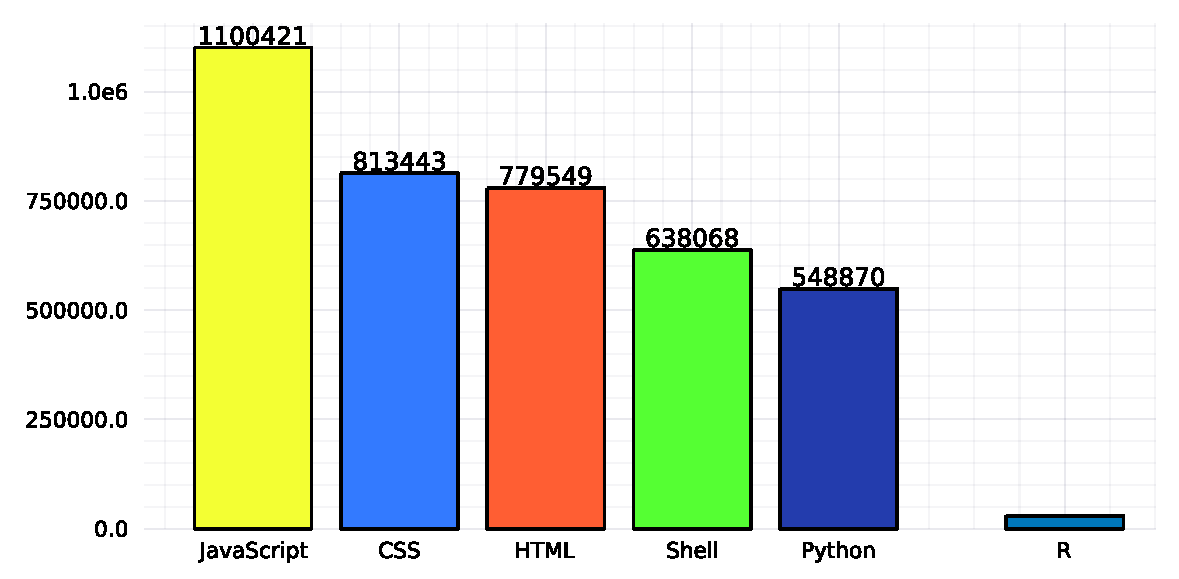
\includegraphics{report_files/figure-pdf/cell-3-output-1.pdf}

}

\caption{Top 5 Linguagens em quantidade de repositórios e R}

\end{figure}

Por honestidade, devemos primeiro notar que R é uma linguagem nichada,
portanto nunca foi esperado que fosse ter quantidade de repositórios
próxima as linguagens anteriormente citadas, porém vale a título de
curiosidade.\\
Seguindo a mesma ideia, vamos analisar as top 5 linguagens que possuem
mais prs e issues ao total. Pela Figura~\ref{fig-plt} notamos que o top
3 se mantém o mesmo tanto pr e issues, entretanto para prs, PHP está no
top 5 e em issues está no top 4, outra diferença é que Ruby aparece em
prs ao invés de C\(++\) que aparece nas issues.

\begin{Shaded}
\begin{Highlighting}[]
\NormalTok{p1 }\OperatorTok{=} \FunctionTok{barh}\NormalTok{(pr, [}\StringTok{"\#bd1616"}\NormalTok{, }\StringTok{"\#5b1bb2"}\NormalTok{])}
\NormalTok{p2 }\OperatorTok{=} \FunctionTok{barh}\NormalTok{(issues, [}\StringTok{"\#5b1bb2"}\NormalTok{,}\StringTok{"\#0b08c0"}\NormalTok{])}
           
\FunctionTok{plot}\NormalTok{(p1,p2, layout}\OperatorTok{=}\FloatTok{2}\NormalTok{, title}\OperatorTok{=}\NormalTok{[}\StringTok{"Pr"} \StringTok{"Issues"}\NormalTok{])}
\end{Highlighting}
\end{Shaded}

\begin{figure}[H]

{\centering 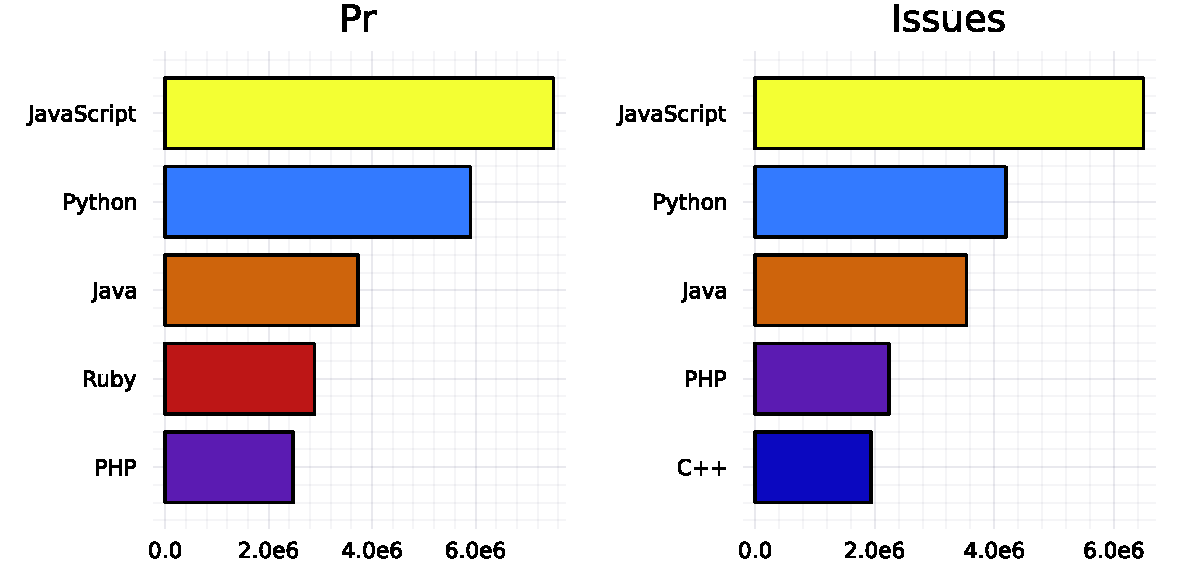
\includegraphics{report_files/figure-pdf/fig-plt-output-1.pdf}

}

\caption{\label{fig-plt}Top 5 Linguagens em quantidade de prs e issues}

\end{figure}

\section{Análise descritiva}

É essencial começar avaliando o comportamento médio de prs e issues no
gh ao longo dos \textbf{anos}. Notamos alguns pontos fundamentais, tanto
prs e issues crescem até atingir seu ápice em 2017, mas os prs
diferentes das issues não descressem de forma monótona depois de 2017.

\begin{Shaded}
\begin{Highlighting}[]
\NormalTok{p1 }\OperatorTok{=} \PreprocessorTok{@pipe} \FunctionTok{top\_5}\NormalTok{(pr,}\OperatorTok{:}\NormalTok{year)  }\OperatorTok{|\textgreater{}}
           \FunctionTok{areaplot}\NormalTok{(\_[}\OperatorTok{:}\NormalTok{,}\OperatorTok{:}\NormalTok{year],\_[}\OperatorTok{:}\NormalTok{,}\OperatorTok{:}\NormalTok{media], title}\OperatorTok{=}\StringTok{"pr"}\NormalTok{, color }\OperatorTok{=} \StringTok{"\#ff4933"}\NormalTok{, }
\NormalTok{           label}\OperatorTok{=}\ConstantTok{false}\NormalTok{, legend}\OperatorTok{=:}\NormalTok{topleft)}
\NormalTok{p2 }\OperatorTok{=} \PreprocessorTok{@pipe} \FunctionTok{top\_5}\NormalTok{(issues,}\OperatorTok{:}\NormalTok{year) }\OperatorTok{|\textgreater{}} 
           \FunctionTok{areaplot}\NormalTok{(\_[}\OperatorTok{:}\NormalTok{,}\OperatorTok{:}\NormalTok{year],\_[}\OperatorTok{:}\NormalTok{,}\OperatorTok{:}\NormalTok{media], title}\OperatorTok{=}\StringTok{"issues"}\NormalTok{, label}\OperatorTok{=}\ConstantTok{false}\NormalTok{, legend}\OperatorTok{=:}\NormalTok{topleft)}
           
\FunctionTok{plot}\NormalTok{(p1,p2,layout}\OperatorTok{=}\FloatTok{2}\NormalTok{)}
\end{Highlighting}
\end{Shaded}

\begin{figure}[H]

{\centering 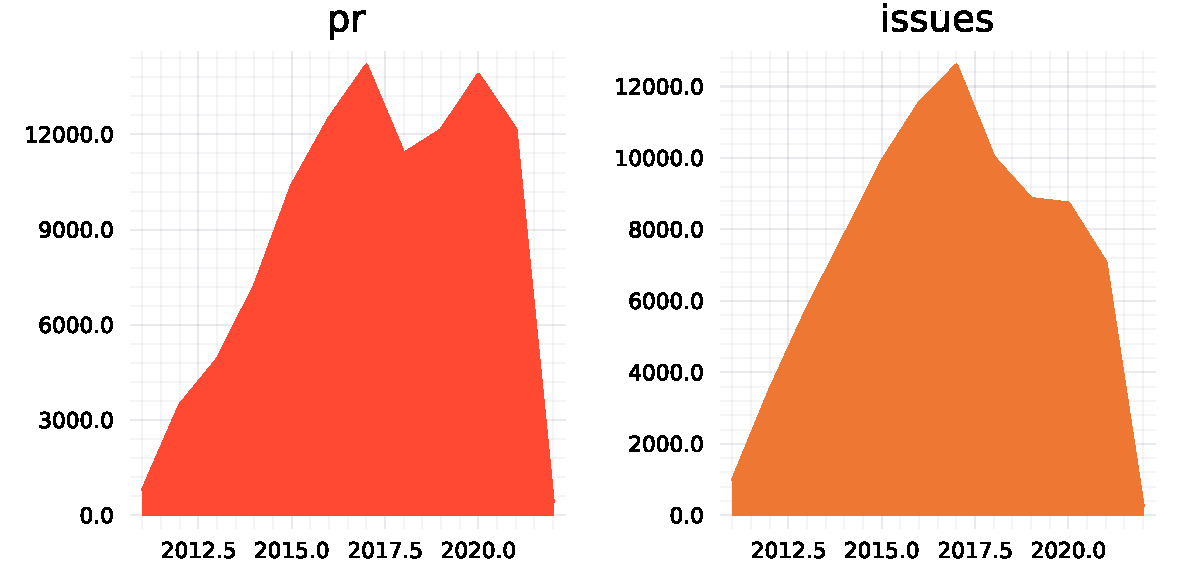
\includegraphics{report_files/figure-pdf/fig-plot-output-1.pdf}

}

\caption{\label{fig-plot}Comportamento médio ao longo dos anos}

\end{figure}

Mas na Figura~\ref{fig-plot}, avaliamos o comportamento das issues e prs
no gh de forma global, independente da linguagem, será que as linguagens
individualmente se comportam da mesma maneira? É isso que veremos nas
seções seguintes

\section{Linguagens Globalmente}

Aqui vamos avaliar o comportamento de 5 linguagens: Java, JavaScript,
PHP, Python e Ruby. Pela Figura~\ref{fig-plot2}, podemos ter um
vislumbre do comportamento de prs para essas linguagens ao longo do
tempo

\begin{Shaded}
\begin{Highlighting}[]
\FunctionTok{fav\_langs}\NormalTok{(pr, [}\StringTok{"Java"}\NormalTok{,}\StringTok{"Python"}\NormalTok{, }\StringTok{"JavaScript"}\NormalTok{, }\StringTok{"Ruby"}\NormalTok{, }\StringTok{"PHP"}\NormalTok{]) }\OperatorTok{|\textgreater{}} 
\NormalTok{      df }\OperatorTok{{-}\textgreater{}} \FunctionTok{plot}\NormalTok{(df[}\OperatorTok{:}\NormalTok{,}\OperatorTok{:}\NormalTok{year], df[}\OperatorTok{:}\NormalTok{,}\OperatorTok{:}\NormalTok{media], g }\OperatorTok{=}\NormalTok{ df[}\OperatorTok{:}\NormalTok{,}\OperatorTok{:}\NormalTok{name])}
\end{Highlighting}
\end{Shaded}

\begin{figure}[H]

{\centering 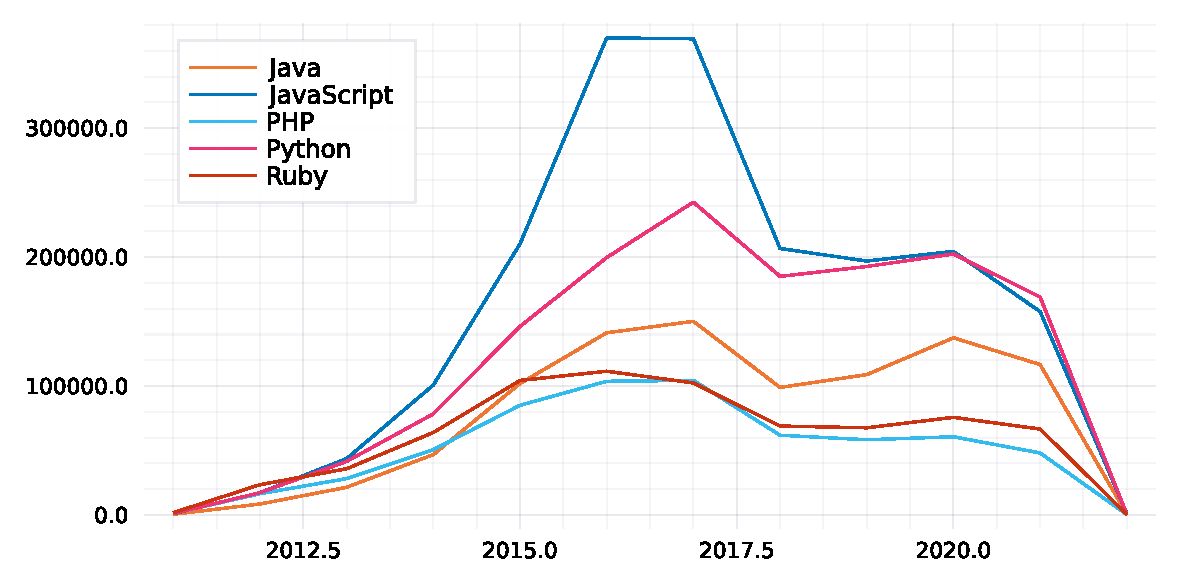
\includegraphics{report_files/figure-pdf/fig-plot2-output-1.pdf}

}

\caption{\label{fig-plot2}Comportamento médio de prs}

\end{figure}

JavaScript domina desde o começo, porém Python avançou muito nos últimos
anos, e em 2021 finalmente ultrapassou JavaScript, outra linguagem que
andou tendo um decréscimo considerável é PHP. Vale ressaltar o pico de
todas as linguagens em 2017, e depois um levo decréscimo, mas somente
PHP e Ruby continuaram caindo consideravelmente nos últimos anos. Pela
Figura~\ref{fig-plot3}, nota-se que Ruby tem um comportamento diferente
em termos de issues que em prs, pois fica abaixo de todas as linguagens
praticamente em todos os anos, Java para issues está mais próximo de
Python do que estava em termos de prs, e Java depois de 2017 só decresce
em issues, algo que não aconteceu em prs.

\begin{Shaded}
\begin{Highlighting}[]
\FunctionTok{fav\_langs}\NormalTok{(issues, [}\StringTok{"Java"}\NormalTok{,}\StringTok{"Python"}\NormalTok{, }\StringTok{"JavaScript"}\NormalTok{, }\StringTok{"Ruby"}\NormalTok{, }\StringTok{"PHP"}\NormalTok{]) }\OperatorTok{|\textgreater{}} 
\NormalTok{      df }\OperatorTok{{-}\textgreater{}} \FunctionTok{plot}\NormalTok{(df[}\OperatorTok{:}\NormalTok{,}\OperatorTok{:}\NormalTok{year], df[}\OperatorTok{:}\NormalTok{,}\OperatorTok{:}\NormalTok{media], g }\OperatorTok{=}\NormalTok{ df[}\OperatorTok{:}\NormalTok{,}\OperatorTok{:}\NormalTok{name])}
\end{Highlighting}
\end{Shaded}

\begin{figure}[H]

{\centering 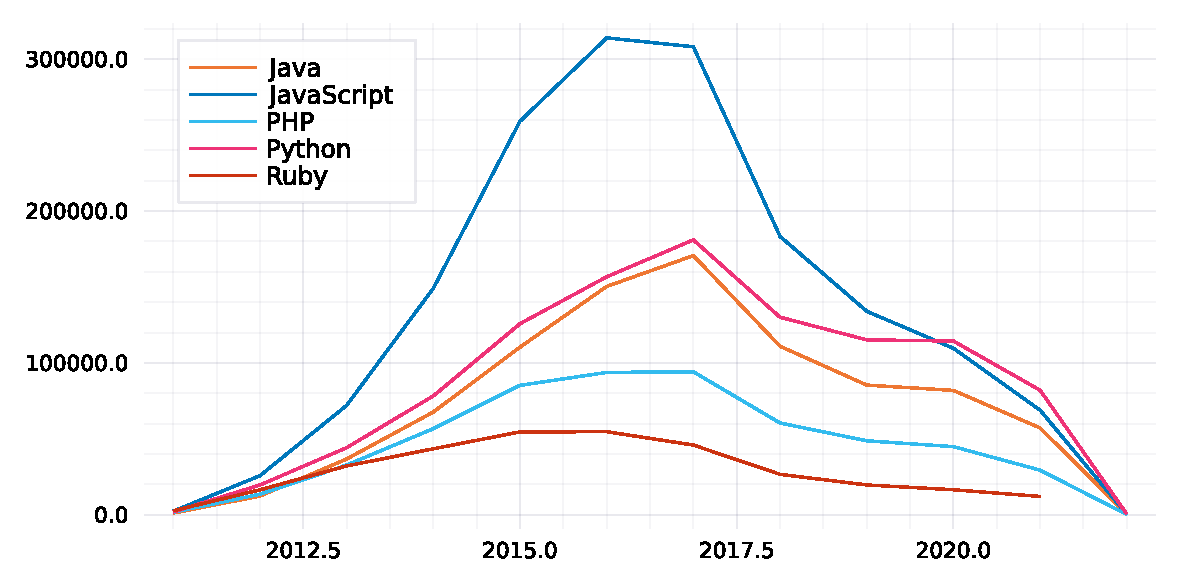
\includegraphics{report_files/figure-pdf/fig-plot3-output-1.pdf}

}

\caption{\label{fig-plot3}Comportamento médio de issues}

\end{figure}

Notamos portanto, um comportamento bem claro, prs cresceram até atingir
seu apogeu em 2017, aonde depois em geral, tendem a cair, as únicas
linguagens das estudadas que recuperaram crescimento foram Java e
Python. Como vimos antes na análise global, as issues somente decrescem
depois de 2017 e o mesmo aconteceu individualmente para as linguagens
estudadas aqui.\\
Vimos que issues decrescem a partir de 2017 monotonicamente de forma
geral e também para as linguagens estudadas nessa subseção, a seguinte
tabela portanto nos informa quais as 5 linguagens mantiveram mais anos
de crescimento após 2017.

\begin{Shaded}
\begin{Highlighting}[]
\NormalTok{lagged }\OperatorTok{=} \PreprocessorTok{@pipe}\NormalTok{ issues[issues.year}\OperatorTok{.\textgreater{}}\FloatTok{2016}\NormalTok{, }\OperatorTok{:}\NormalTok{] }\OperatorTok{|\textgreater{}}
               \FunctionTok{groupby}\NormalTok{(\_, [}\OperatorTok{:}\NormalTok{year, }\OperatorTok{:}\NormalTok{name]) }\OperatorTok{|\textgreater{}}
               \FunctionTok{combine}\NormalTok{(\_, }\OperatorTok{:}\NormalTok{count }\OperatorTok{=\textgreater{}}\NormalTok{ mean) }\OperatorTok{|\textgreater{}}
               \FunctionTok{groupby}\NormalTok{(\_, }\OperatorTok{:}\NormalTok{name) }\OperatorTok{|\textgreater{}}
               \FunctionTok{combine}\NormalTok{(\_, }\OperatorTok{:}\NormalTok{count\_mean }\OperatorTok{=\textgreater{}}\NormalTok{ (lag }\OperatorTok{=\textgreater{}} \OperatorTok{:}\NormalTok{count));}
\NormalTok{lagged[}\OperatorTok{:}\NormalTok{, }\OperatorTok{:}\NormalTok{count] }\OperatorTok{=}  \FunctionTok{ifelse}\NormalTok{.(lagged[}\OperatorTok{:}\NormalTok{, }\OperatorTok{:}\NormalTok{count] }\OperatorTok{.\textgreater{}} \FloatTok{0}\NormalTok{, }\FloatTok{1}\NormalTok{, }\FloatTok{0}\NormalTok{);}
\end{Highlighting}
\end{Shaded}

\begin{table}[H]
\centering
\begin{tabular}[t]{c|c}
\hline
Linguagem & Total de crescimento\\
\hline
ColdFusion & 3\\
\hline
Dart & 3\\
\hline
Nunjucks & 3\\
\hline
ActionScript & 2\\
\hline
Go & 2\\
\hline
\end{tabular}
\caption{Top 5 Linguagens em quantidade de crescimento em issues após 2017.}
\end{table}

Das 5 linguagens, 3 tiveram 3 anos de crescimento de issues se comparado
ao ano anterior, ou seja: \textbf{nenhuma} linguagem permaneceu somente
crescendo em issues após 2017.

\section{Linguagens para Dados}

Nessa seção vamos avaliar o comportamento especificamente de R e Julia,
que são duas das três principais linguagens para trabalhar com dados no
momento.

\subsection{Breve Introdução}

R é uma implementação open-source da Linguagem
\href{https://en.wikipedia.org/wiki/S_(programming_language)}{S}, teve
seu lançamento oficial em 1995, sendo desenvolvida por
\href{https://en.wikipedia.org/wiki/Ross_Ihaka}{Ross Ihaka} e
\href{https://en.wikipedia.org/wiki/Robert_Gentleman_(statistician)}{Robert
Gentleman}, sendo assim seu nome ``R'' vem da letra inicial do seus
criadores e também do dialeto com ``S''. R tem suas raízes na
estatística computacional, passou seus 10 primeiros anos sendo
primariamente uma linguagem acadêmica, mas depois do desenvolvimento de
pacotes como \texttt{tidyverse} se tornou um ambiente propicio para
ciência de dados.

O projeto da linguagem Julia teve seu início em meados de 2009, muitos
dos seus criadores usavam certas ferramentas que funcionavam para
tarefas especificas mas em outras eram terríveis, portanto Julia surge
sendo uma linguagem que deveria aglomerar tudo que certas linguagens
faziam de bom, como ser rápida como C, ser boa em estatística como o R,
ser de proposito geral como Python, ser poderosa em algebra linear como
Matlab, e repetindo ser \textbf{rápida} como C, sendo assim, foi lançada
oficialmente em 2012, no momento que o autor vos escreve, Julia está
fazendo 10 anos, mesmo com somente 10 anos de idade Julia já é usada
pela NASA e também pelo INPE.\\
Vamos começar avaliando a quantidade total de repositórios para cada uma
das duas linguagens.

\begin{Shaded}
\begin{Highlighting}[]
\NormalTok{total[}\FunctionTok{findall}\NormalTok{(}\FunctionTok{in}\NormalTok{([}\StringTok{"R"}\NormalTok{, }\StringTok{"Julia"}\NormalTok{]), total[}\OperatorTok{:}\NormalTok{, }\OperatorTok{:}\NormalTok{language]), }\OperatorTok{:}\NormalTok{] }\OperatorTok{|\textgreater{}}
\NormalTok{df }\OperatorTok{{-}\textgreater{}} \FunctionTok{super\_bar}\NormalTok{(df, }\OperatorTok{:}\NormalTok{language, }\OperatorTok{:}\NormalTok{num\_repos,[}\StringTok{"\#2B5FE9"}\NormalTok{, }\StringTok{"\#AA30FF"}\NormalTok{])}
\end{Highlighting}
\end{Shaded}

\begin{figure}[H]

{\centering 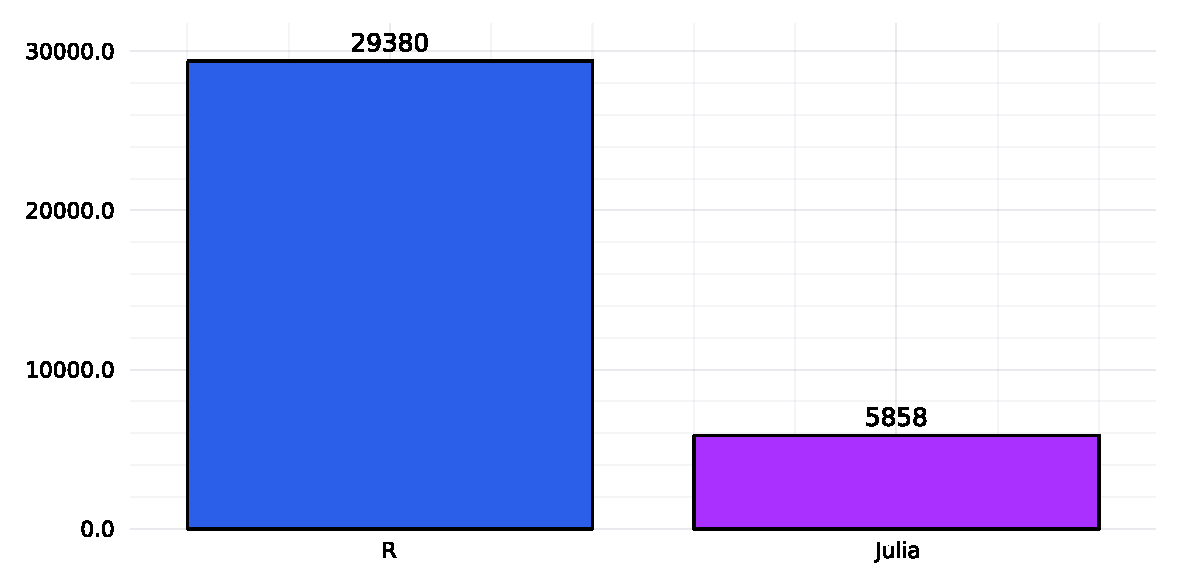
\includegraphics{report_files/figure-pdf/cell-9-output-1.pdf}

}

\caption{Quantidade de repositórios disponíveis para R e Julia}

\end{figure}

Podemos ver que R possui muito mais repositórios disponíveis no gh,
porém R é uma linguagem que está a bastante tempo no mercado, ao
contrário de Julia. Como dito anteriormente, R nos seus primeiros anos
foi uma linguagem primariamente acadêmica, isso significa que a maioria
dos seus repositórios são para ferramentas para a própria linguagem, e é
nessa fase que Julia se situa atualmente.

Agora vamos ver o comportamento das duas linguagens ao longo dos últimos
anos

\begin{Shaded}
\begin{Highlighting}[]
\NormalTok{p1 }\OperatorTok{=} \FunctionTok{fav\_langs}\NormalTok{(pr, [}\StringTok{"R"}\NormalTok{,}\StringTok{"Julia"}\NormalTok{]) }\OperatorTok{|\textgreater{}} 
\NormalTok{      df }\OperatorTok{{-}\textgreater{}} \FunctionTok{plot}\NormalTok{(df[}\OperatorTok{:}\NormalTok{,}\OperatorTok{:}\NormalTok{year], df[}\OperatorTok{:}\NormalTok{,}\OperatorTok{:}\NormalTok{media], g }\OperatorTok{=}\NormalTok{ df[}\OperatorTok{:}\NormalTok{,}\OperatorTok{:}\NormalTok{name], title }\OperatorTok{=} \StringTok{"Pull Requests"}\NormalTok{)}
\NormalTok{p2 }\OperatorTok{=} \FunctionTok{fav\_langs}\NormalTok{(issues, [}\StringTok{"R"}\NormalTok{,}\StringTok{"Julia"}\NormalTok{]) }\OperatorTok{|\textgreater{}} 
\NormalTok{      df }\OperatorTok{{-}\textgreater{}} \FunctionTok{plot}\NormalTok{(df[}\OperatorTok{:}\NormalTok{,}\OperatorTok{:}\NormalTok{year], df[}\OperatorTok{:}\NormalTok{,}\OperatorTok{:}\NormalTok{media], g }\OperatorTok{=}\NormalTok{ df[}\OperatorTok{:}\NormalTok{,}\OperatorTok{:}\NormalTok{name], title }\OperatorTok{=} \StringTok{"Issues"}\NormalTok{)}

\FunctionTok{plot}\NormalTok{(p1,p2,layout}\OperatorTok{=}\NormalTok{(}\FloatTok{1}\NormalTok{,}\FloatTok{2}\NormalTok{))}
\end{Highlighting}
\end{Shaded}

\begin{figure}[H]

{\centering 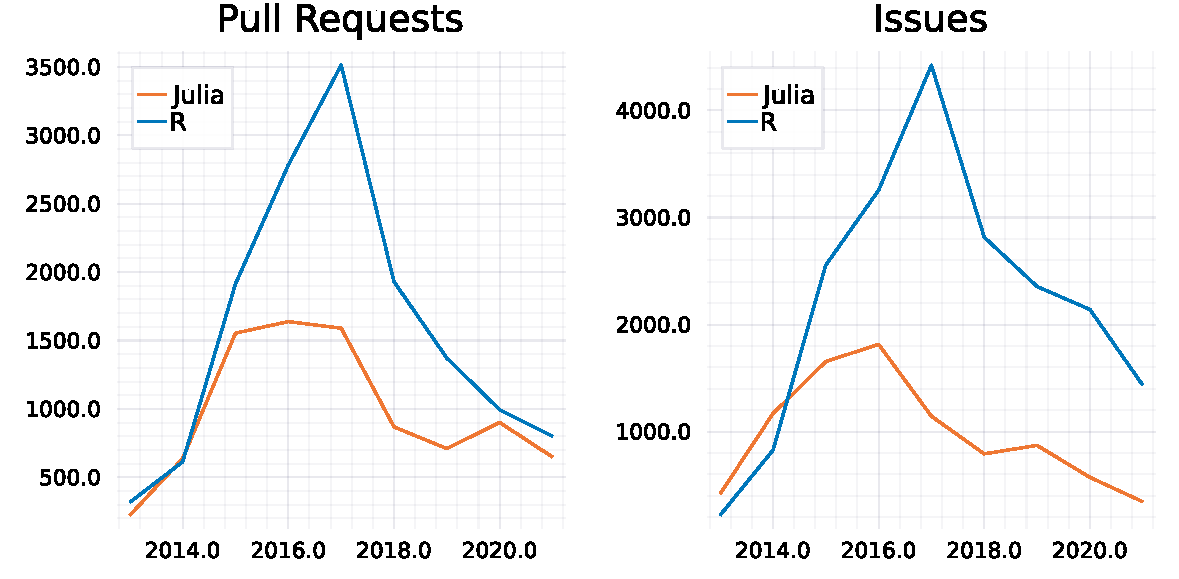
\includegraphics{report_files/figure-pdf/cell-10-output-1.pdf}

}

\caption{Média de prs e issues para R e Julia}

\end{figure}

Nota-se que em 2014 Julia teve mais prs e issues que R e ambas as
linguagens atingem seu pico em 2017, um comportamento global como vimos
anteriormente, porém para issues Julia teve mais de 2012 até 2014 e
também seu pico de issues foi em 2016 e não 2017 como R.

\subsection{Python entra no game}

Evidentemente não podemos esquecer de Python, pois como vimos está no
top 5 de linguagens com mais repositórios disponíveis, atualmente conta
com vários pacotes para análise de dados, e é a principal linguagem para
deep learning, então é claro que não poderia faltar a comparação com
suas concorrentes nesse ramo. Notamos que há uma diferença
desproporcional em termos de prs e issues a comparação com R e Julia.

\begin{Shaded}
\begin{Highlighting}[]
\NormalTok{p1 }\OperatorTok{=} \FunctionTok{fav\_langs}\NormalTok{(pr, [}\StringTok{"R"}\NormalTok{,}\StringTok{"Julia"}\NormalTok{,}\StringTok{"Python"}\NormalTok{]) }\OperatorTok{|\textgreater{}} 
\NormalTok{      df }\OperatorTok{{-}\textgreater{}} \FunctionTok{plot}\NormalTok{(df[}\OperatorTok{:}\NormalTok{,}\OperatorTok{:}\NormalTok{year], df[}\OperatorTok{:}\NormalTok{,}\OperatorTok{:}\NormalTok{media], g }\OperatorTok{=}\NormalTok{ df[}\OperatorTok{:}\NormalTok{,}\OperatorTok{:}\NormalTok{name])}
\NormalTok{p2 }\OperatorTok{=} \FunctionTok{fav\_langs}\NormalTok{(issues, [}\StringTok{"R"}\NormalTok{,}\StringTok{"Julia"}\NormalTok{, }\StringTok{"Python"}\NormalTok{]) }\OperatorTok{|\textgreater{}} 
\NormalTok{      df }\OperatorTok{{-}\textgreater{}} \FunctionTok{plot}\NormalTok{(df[}\OperatorTok{:}\NormalTok{,}\OperatorTok{:}\NormalTok{year], df[}\OperatorTok{:}\NormalTok{,}\OperatorTok{:}\NormalTok{media], g }\OperatorTok{=}\NormalTok{ df[}\OperatorTok{:}\NormalTok{,}\OperatorTok{:}\NormalTok{name])}

\FunctionTok{plot}\NormalTok{(p1,p2,layout}\OperatorTok{=}\NormalTok{(}\FloatTok{1}\NormalTok{,}\FloatTok{2}\NormalTok{))}
\end{Highlighting}
\end{Shaded}

\begin{figure}[H]

{\centering 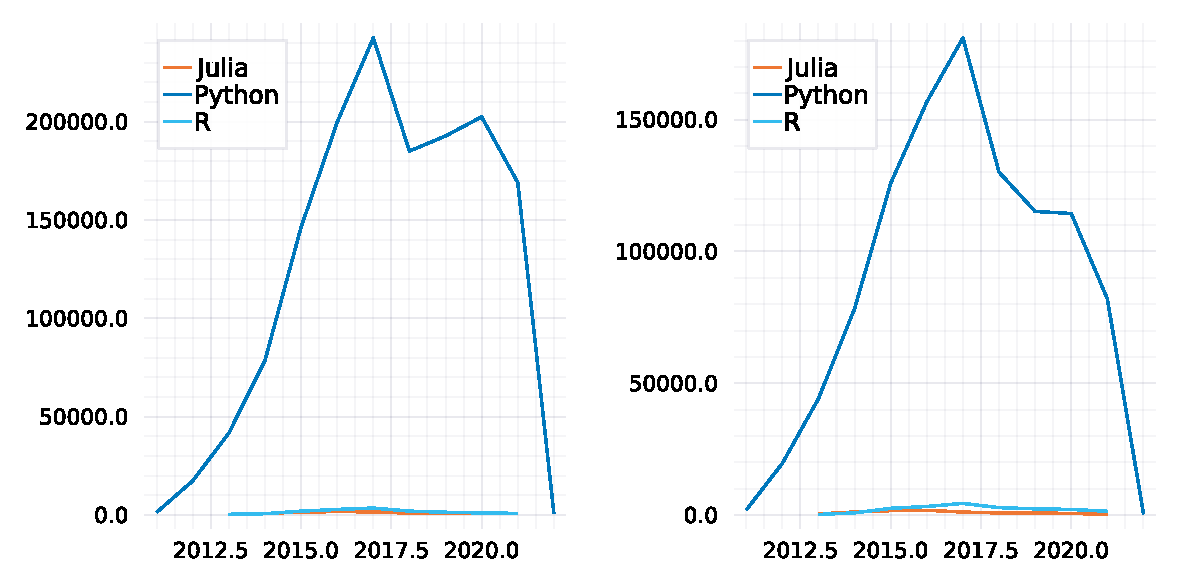
\includegraphics{report_files/figure-pdf/cell-11-output-1.pdf}

}

\end{figure}

Sabemos que Python é de proposito geral e uma linguagem bem
estabelecida, então evidentemente tende a ocupar mais espaço que R e
Julia. Um ponto fundamental, é que se filtrarmos em repositórios com
vies de análise de dados/ machine learning, será que Python tende a
manter essa distância das outras linguagens? Infelizmente tal filtragem
seria puramente arbitrária, pois como definimos o que é um repositório
de análise de dados? Qualquer maneira de definir pode facilmente não
incluir pontos relevantes, assim a resposta para a pergunta anterior
fica a cargo do leitor.

\section{Conclusão momentânea}

Vimos que JavaScript leva vantagem de todas as linguagens em todos os
anos, e também fica claro a discrepância que JavaScript tem das outras
linguagens, pois pela Figura~\ref{fig-plot} vemos que o valor médio
geral para pr e issues é muito inferior que o de JavaScript, Python vem
brigando pela superioridade com JavaScript ao longo dos anos, sendo que
em 2021 o superou nas métricas estudadas aqui. Vimos também que Julia é
uma linguagem nova e em ascensão, pois atualmente ela está na fase em
que R se encontrava a 10 anos atrás, porém já possuindo algumas
aplicações no mercado. Python tem muito destaque sobre as outras
linguagens que tem viés para análise de dados, mas vale ressaltar que
python não nasceu com esse propósito.\\
Será que o que observamos aqui vai se manter daqui 10 anos? Será que a
linguagem Julia tem potencial para superar R e Python? Python vai
continuar em ascensão? São muitas perguntas e no momento poucas
respostas, só o tempo e empenho das comunidades trarão as respostas
desejadas.



\end{document}
